%%%%%%%%%%%%%%%%%%%%%%%%%%%%%%%%%%%%%%%%%%%%%%%%
%% Compile: PDFLaTeX BibTeX PDFLaTeX PDFLaTeX
%% Course Slides: Wissenschaftliches Arbeiten
%% Antonio Machicao y Priemer
%%%%%%%%%%%%%%%%%%%%%%%%%%%%%%%%%%%%%%%%%%%%%%%%

\documentclass[a4paper,10pt, bibtotoc]{beamer}
%\documentclass[a4paper,10pt,handout]{beamer}

%%%%%%%%%%%%%%%%%%%%%%%%%
%% PACKAGES & COMMANDS 
%%%%%%%%%%%%%%%%%%%%%%%%%

%%%%%%%%%%%%%%%%%%%%%%%%%%%%%%%%%%%%%%%%%%%%%%%%%%%%
%%%          MyP-Packages   2018.12.08    XeLaTeX
%%%%%%%%%%%%%%%%%%%%%%%%%%%%%%%%%%%%%%%%%%%%%%%%%%%%


%\usepackage[utf8]{inputenc} %XeLaTeX

%% For German texts
\usepackage[ngerman,english]{babel}

%% For English texts
%\usepackage[ngerman,english]{babel}

%% Captions numbered in Beamer 
\setbeamertemplate{caption}[numbered]

%% Change ''Abbildung'' into ''Abb.'' 
%% for: babel
	\renewcommand{\thefigure}{\arabic{figure}}
	\addto\captionsngerman{%
		\renewcommand{\figurename}{Abb.}%
	}
	\renewcommand{\figurename}{Abb.} 

%% Change ''Figure'' into ''Fig.'' 
%% for: babel
	\renewcommand{\thefigure}{\arabic{figure}}
	\addto\captionsenglish{%
		\renewcommand{\figurename}{Fig.}%
	}
%	\renewcommand{\figurename}{Fig.} %% << not needed? 


%% TIPA encoding needs options: T3 & T1
\usepackage[T3,T1]{fontenc}  %not needed in XeLaTeX (?)

%\usepackage{fontspec} % XeLaTeX: Problem: Libertine+Fontspec+TIPA

%% Font
\usepackage{lmodern}
%\usepackage{libertine} % XeLaTeX: Problem: Libertine+Fontspec+TIPA

%% Blind text: \blindtext \Blindtext \blindtext[5] \blindlist{itemize}[x] ...
\usepackage{blindtext}

%% ulem: Strike out
\usepackage[normalem]{ulem}  

%% graphicx: if gb4e is active PDFLaTeX does not accept files with underline. PDFLaTeX accepts files only with .jpg, .png, .pdf endings
\usepackage{graphicx}

%% Math symbols
\usepackage{amsmath}
\usepackage{amsfonts}
\usepackage{amssymb}
\usepackage{MnSymbol} 				% Meaning brackets 

%% Toggles
\usepackage{etoolbox}
	\newtoggle{handout}


%%%%%%%%%%%%%%%%%%%%%%%%%%%%%%%%%%%%%%%%%%%%%%%%%%%%
%%%         Tables & Lists & Columns            
%%%%%%%%%%%%%%%%%%%%%%%%%%%%%%%%%%%%%%%%%%%%%%%%%%%%

% Text in columns: \begin{multicols}{n} \columnbreak \end{multicols}
\usepackage{multicol}
%	\setlength{\columnsep}{.5cm}	

%% Tables with specified width
\usepackage{tabularx}

%% For complex tables
\usepackage{array}

%% For other tables
\usepackage{booktabs}

%% For more than one row in a table
\usepackage{multirow}

%% Special lists: itemize*
\usepackage{mdwlist}


%%%%%%%%%%%%%%%%%%%%%%%%%%%%%%%%%%%%%%%%%%%%%%%%%%%%
%%%          Coloured elements                  
%%%%%%%%%%%%%%%%%%%%%%%%%%%%%%%%%%%%%%%%%%%%%%%%%%%%
%Use xcolor before `gb4e'!
\usepackage{xcolor}


%%%%%%%%%%%%%%%%%%%%%%%%%%%%%%%%%%%%%%%%%%%%%%%%%%%%
%%%          Trees                               
%%%%%%%%%%%%%%%%%%%%%%%%%%%%%%%%%%%%%%%%%%%%%%%%%%%%
%% Forest must be loaded before `gb4e'
\usepackage{forest}
	
	%% Needed for the "actual forest version"
	\useforestlibrary{linguistics}
	\forestapplylibrarydefaults{linguistics}

%% Old forest version
%\usepackage{etex}		%For Forest bug
%\usepackage{../forestold}
	
	
%%%%%%%%%%%%%%%%%%%%%%%%%%%%%%%%%%%%%%%%%%%%%%%%%%%%
%%%          Venndiagram                         
%%%%%%%%%%%%%%%%%%%%%%%%%%%%%%%%%%%%%%%%%%%%%%%%%%%%
%% Package needed: tikz
\usepackage{venndiagram}


%%%%%%%%%%%%%%%%%%%%%%%%%%%%%%%%%%%%%%%%%%%%%%%%%%%%%
%%%%          Verbatim                            
%%%%%%%%%%%%%%%%%%%%%%%%%%%%%%%%%%%%%%%%%%%%%%%%%%%%%
%%`Listings' must be loaded before `gb4', use `verbatim' otherwise
\usepackage{listings}

\lstset{
	language=TeX,
	backgroundcolor=\color{lightgray},
	basicstyle={\footnotesize\ttfamily\color{blue}},
	showstringspaces=false,
	columns=flexible
}
\lstset{literate=%
	{Ö}{{\"O}}1
	{Ä}{{\"A}}1
	{Ü}{{\"U}}1
	{ß}{{\ss}}2
	{ü}{{\"u}}1
	{ä}{{\"a}}1
	{ö}{{\"o}}1
}

%\lstset{%frame=tb,
%	language=Perl,
%	aboveskip=3mm,
%	belowskip=3mm,
%	showstringspaces=false,
%	columns=flexible,
%	basicstyle={\small\ttfamily\color{blue}},
%	numbers=none,
%	%numberstyle=\tiny\color{gray},
%	extendedchars=false,
%	morekeywords={foo},
%	otherkeywords={\#\#},
%	%keywordstyle=\color{blau},
%	%commentstyle=\color{whiteblue},
%	%stringstyle=\color{mauve},
%	breaklines=true,
%	breakatwhitespace=true,
%	tabsize=3
%}


%%%%%%%%%%%%%%%%%%%%%%%%%%%%%%%%%%%%%%%%%%%%%%%%%%%%%
%%%%       Attribute Value Matrices               
%%%%%%%%%%%%%%%%%%%%%%%%%%%%%%%%%%%%%%%%%%%%%%%%%%%%%
\usepackage{../../texfiles-beamer/avm}
%%% Setting of avm (see LSP Guidelines)
	%	\avmfont{\sc}
	%	\avmvalfont{\it}
	\avmfont{\normalfont \scshape} 
	\avmvalfont{\normalfont \itshape} 
%% command to fontify the type values of an avm 
	\newcommand{\tpv}[1]{{\avmjvalfont #1}} 
%% command to fontify the type of an avm and avmspan it
	\newcommand{\tp}[1]{\avmspan{\tpv{#1}}}


%%%%%%%%%%%%%%%%%%%%%%%%%%%%%%%%%%%%%%%%%%%%%%%%%%%%
%%%          IPA                                 
%%%%%%%%%%%%%%%%%%%%%%%%%%%%%%%%%%%%%%%%%%%%%%%%%%%%
%\usepackage[noenc,safe]{tipa}	%in PDFLaTeX
\usepackage[safe]{tipa}	% in XeLaTeX


%%%%%%%%%%%%%%%%%%%%%%%%%%%%%%%%%%%%%%%%%%%%%%%%%%%%
%%%          Vowel diagram                       
%%%%%%%%%%%%%%%%%%%%%%%%%%%%%%%%%%%%%%%%%%%%%%%%%%%%
%\usepackage{vowel}


%%%%%%%%%%%%%%%%%%%%%%%%%%%%%%%%%%%%%%%%%%%%%%%%%%%%
%%%          Bibliography                        
%%%%%%%%%%%%%%%%%%%%%%%%%%%%%%%%%%%%%%%%%%%%%%%%%%%%
\usepackage{natbib}	
	\setcitestyle{notesep={:~}}


%%%%%%%%%%%%%%%%%%%%%%%%%%%%%%%%%%%%%%%%%%%%%%%%%%%%%
%%%%          Settings of the page                
%%%%%%%%%%%%%%%%%%%%%%%%%%%%%%%%%%%%%%%%%%%%%%%%%%%%%

%% (Vertical) Spacing
\usepackage{setspace}
%	\onehalfspacing

%% Space for abbreviations 'i.d.R'
\usepackage{xspace}

%% Margins % >> Option clash for beamer
%\usepackage[a4paper]{geometry} 	
%	\geometry{top=2.5cm, bottom=2.5cm, left=2.5cm, right=2.5cm}


%%%%%%%%%%%%%%%%%%%%%%%%%%%%%%%%%%%%%%%%%%%%%%%%%%%%%
%%%%          Margin notes                        
%%%%%%%%%%%%%%%%%%%%%%%%%%%%%%%%%%%%%%%%%%%%%%%%%%%%%
%% See definition in localcommands.sty, not working with Beamer class
%\usepackage{marginnote}


%%%%%%%%%%%%%%%%%%%%%%%%%%%%%%%%%%%%%%%%%%%%%%%%%%%%%%
%%%%%                Videos                        
%%%%%%%%%%%%%%%%%%%%%%%%%%%%%%%%%%%%%%%%%%%%%%%%%%%%%%
%%Embedding videos >> it does not work
%\usepackage{media9} 


%%%%%%%%%%%%%%%%%%%%%%%%%%%%%%%%%%%%%%%%%%%%%%%%%%%%
%%%          Hyperref & URL                      
%%%%%%%%%%%%%%%%%%%%%%%%%%%%%%%%%%%%%%%%%%%%%%%%%%%%

%\usepackage[hyphens]{url}
\usepackage{url}

%\usepackage{hyperref}

%\usepackage[
%	bookmarksnumbered, % For numbered bookmarks in PDF, not needed for Beamer class
%	hidelinks, %For links without colored borders
%	hyperfootnotes=false %If FNs takes you to the 1st page and not to the FN text
%	]{hyperref}


%%%%%%%%%%%%%%%%%%%%%%%%%%%%%%%%%%%%%%%%%%%%%%%%%%%%
%%%           Examples                           
%%%%%%%%%%%%%%%%%%%%%%%%%%%%%%%%%%%%%%%%%%%%%%%%%%%%

%%% Easy to use: 
%\usepackage{linguex}

%%% gb4e: more powerful than linguex, but with many bugs.
%%% Add gb4e as one of the last packages! 
%\usepackage{gb4e}

%% lsp-gb4eMyP: lsp-Variant of gb4e by MyP
\usepackage{../../texfiles-beamer/lsp-gb4eMyP}

%% (for lsp-gb4eMyP: to add additional information to the right of examples, uncomment the following line)
\usepackage{../../texfiles-beamer/jambox}
%	\jamwidth=2cm\relax 

%% (for lsp-gb4eMyP: if you want the source line of examples to be in italics, uncomment the following line)
% \def\exfont{\it}		


%%%%%%%%%%%%%%%%%%%%%%%%%%%%%%%%%%%%%%%%%%%%%%%%%%%%
%%%           Style Sheet HU                     %%%
%%%%%%%%%%%%%%%%%%%%%%%%%%%%%%%%%%%%%%%%%%%%%%%%%%%%
%% huberlin: Style sheet
\usepackage{../../texfiles-beamer/tex-styleHU/huberlin}

%%% Uni-Tuebingen: Style sheet
%\usepackage{../../texfiles-beamer/tex-styleHU/unituebingen}

%%%%%%%%%%%%%%%%%%%%%%%%%%%%%%%%%%%%%%%%%%%%%%%%%%%%
%%%           MyP-Commands  2018.12.08       
%%%%%%%%%%%%%%%%%%%%%%%%%%%%%%%%%%%%%%%%%%%%%%%%%%%%   


%%%%%%%%%%%%%%%%%%%%%%%%%%%%%%%%
% German quotation marks:
\newcommand{\gqq}[1]{\glqq{}#1\grqq{}}		%double
\newcommand{\gq}[1]{\glq{}#1\grq{}}			%simple


%%%%%%%%%%%%%%%%%%%%%%%%%%%%%%%%
% Abbreviations in German
% package needed: xspace
% Short space in German abbreviations: \,	
\newcommand{\dash}{\mbox{d.\,h.}\xspace}
\newcommand{\idR}{\mbox{i.\,d.\,R.}\xspace}
\newcommand{\su}{\mbox{s.\,u.}\xspace}
\newcommand{\ua}{\mbox{u.\,a.}\xspace}
\newcommand{\va}{\mbox{v.\,a.}\xspace}
\newcommand{\zB}{\mbox{z.\,B.}\xspace}
%\newcommand{\s}{s.~}
%not possibel: \dh --> d.\,h.


%%%%%%%%%%%%%%%%%%%%%%%%%%%%%%%%
%Abbreviations in English
\newcommand{\ao}{a.o.\ }	% among others
\newcommand{\cf}[1]{(cf.~#1)}	% confer = compare
\newcommand{\cfe}[1]{(cf.~(\ref{#1}))}	% compare + example
\newcommand{\ia}{i.a.}	% inter alia = among others
\newcommand{\ie}{i.e.~}	% id est = that is
\newcommand{\fe}{e.g.~}	% exempli gratia = for example
%not possible: \eg --> e.g.~
\newcommand{\vs}{vs.\ }	% versus
\newcommand{\wrt}{w.r.t.\ }	% with respect to


%%%%%%%%%%%%%%%%%%%%%%%%%%%%%%%%
% Dash:
\newcommand{\gs}[1]{--\,#1\,--}


%%%%%%%%%%%%%%%%%%%%%%%%%%%%%%%%
% Rightarrow with and without space
\def\ra{\ensuremath\rightarrow}			%without space
\def\ras{\ensuremath\rightarrow\ }		%with space
\def\la{\ensuremath\leftarrow}
\def\las{\ensuremath\leftarrow\ }


%%%%%%%%%%%%%%%%%%%%%%%%%%%%%%%%
%% X-bar notation

%% Notation with primes (not emphasized): \xprime{X}
\newcommand{\xprime}[1]{#1$^{\prime}$}
\newcommand{\xxprime}[1]{#1$^{\prime\prime}$}
\newcommand{\xxxprime}[1]{#1$^{\prime\prime\prime}$}

%% Notation with primes (emphasized): \exbar{X}
\newcommand{\exprime}[1]{\emph{#1}$^{\prime}$}
\newcommand{\exxprime}[1]{\emph{#1}$^{\prime\prime}$}
\newcommand{\exxxprime}[1]{\emph{#1}$^{\prime\prime\prime}$}

% Notation with zero and max (not emphasized): \xbar{X}
\newcommand{\xzero}[1]{#1$^{0}$}
\newcommand{\maxbar}[1]{#1$^{\textsc{max}}$}

% Notation with zero and max (emphasized): \xbar{X}
\newcommand{\ezerobar}[1]{\emph{#1}$^{0}$}
\newcommand{\emaxbar}[1]{\emph{#1}$^{\textsc{max}}$}

%% Notation with bars (already implemented in gb4e):
% \obar{X}, \ibar{X}, \iibar{X}, \mbar{X} %Problems with \mbar!
% $\overline{}$
%
%% Without gb4e:
\newcommand{\overbar}[1]{\mkern 1.5mu\overline{\mkern-1.5mu#1\mkern-1.5mu}\mkern 1.5mu}
%
%%% OR:
%\newcommand{\ibar}[1]{$\overline{\textrm{#1}}$}
%\newcommand{\iibar}[1]{$\overline{\overline{\textrm{#1}}}$}
%% (emphasized):
\newcommand{\eibar}[1]{$\overline{#1}$}
\newcommand{\eiibar}[1]{\overline{$\overline{#1}}$}


%%%%%%%%%%%%%%%%%%%%%%%%%%%%%%%%
%% Subscript & Superscript: no italics inside math mode
\newcommand{\down}[1]{\textsubscript{#1}}
\newcommand{\downm}[1]{_{\textrm{#1}}}

\newcommand{\up}[1]{\textsuperscript{#1}}
\newcommand{\upm}[1]{^{\textrm{#1}}}


%%%%%%%%%%%%%%%%%%%%%%%%%%%%%%%%
%% Small caps subscripts
\newcommand{\scdown}[1]{\textsubscript{\textsc{#1}}}


%%%%%%%%%%%%%%%%%%%%%%%%%%%%%%%%%
%%% Shorter Underline
%\DeclareTextCommand{\_}{T1}{\leavevmode \kern.06em\vbox{\hrule width.4em}}


%%%%%%%%%%%%%%%%%%%%%%%%%%%%%%%%
%% Object- and Meta-language marking:
%\newcommand{\obj}[1]{\glqq{}#1\grqq{}}		%German double quotes
%\newcommand{\obj}[1]{``#1''}					  %English double quotes
\newcommand{\obj}[1]{\emph{#1}}                 %Emphasising
\newcommand{\term}[1]{\textsc{#1}}              %for abbreviated terminology


%%%%%%%%%%%%%%%%%%%%%%%%%%%%%%%%
% Size:
\newcommand{\size}[1]{{\footnotesize #1}}	% f.e. resize citations


%%%%%%%%%%%%%%%%%%%%%%%%%%%%%%%%
%% for LaTeX terminology: package names, environments, commands
\newcommand{\ltxterm}[1]{{\footnotesize \texttt{#1}}}
\newcommand{\ltxpack}[1]{{\footnotesize \texttt{#1}}}


%%%%%%%%%%%%%%%%%%%%%%%%%%%%%%%%
% Short cuts (<STRG + ALT>):
%\newcommand{\short}[1]{\texttt{\textsc{#1}}}		%Emphasising
\newcommand{\short}[1]{$\langle$\texttt{\textsc{#1}}$\rangle$}		%Emphasising


%%%%%%%%%%%%%%%%%%%%%%%%%%%%%%%%
% Writing text with colour:
% package needed: xcolor
% Command \alert{} in Beamer >> red
\newcommand{\blue}[1]{\textcolor{blue}{#1}}
\newcommand{\green}[1]{\textcolor{green}{#1}}
\newcommand{\red}[1]{\textcolor{red}{#1}}


%%%%%%%%%%%%%%%%%%%%%%%%%%%%%%%%
%% Marking text with colour: 
%%% package needed: color
\newcommand{\clrr}[1]{\colorbox{red}{#1}}
\newcommand{\clry}[1]{\colorbox{yellow}{#1}}


%%%%%%%%%%%%%%%%%%%%%%%%%%%%%%%%
%% Semantic types (<e,t>), features, variables and graphemes in angled brackets 

%%% types and variables, in math mode: angled brackets + italics + no space
%\newcommand{\type}[1]{$<#1>$}

%%% OR more correctly: 
%%% Types and Variables: chevrons! + text in math mode (italics + no space)
\newcommand{\type}[1]{$\langle #1 \rangle$} %% In Math Mode, only single types
\newcommand{\typem}[1]{\langle #1 \rangle } %% Mathmode extra, complex types

%%% Features and Graphemes: chevrons! + normal font
\newcommand{\ab}[1]{$\langle$#1$\rangle$} %% no italics
\newcommand{\abe}[1]{$\langle$\emph{#1}$\rangle$} %% italics


%%%%%%%%%%%%%%%%%%%%%%%%%%%%%%%%
%% Function symbol in Beamer Class!
%% italics and serif
\newcommand{\func}{\emph{\textrm{f}}}
\newcommand{\gunc}{\emph{\textrm{g}}}
\newcommand{\chiF}[1]{\chi _{\textrm{#1}}} 


%%%%%%%%%%%%%%%%%%%%%%%%%%%%%%%%
%% HPSG: Features and Values!
\newcommand{\wert}[1]{\emph{#1}}		%Values & Types
\newcommand{\val}[1]{\emph{#1}}		%Values & Types
\newcommand{\feat}[1]{\textsc{#1}}	%Features


%%%%%%%%%%%%%%%%%%%%%%%%%%%%%%%%
%% (Syntactic) Trees
% package needed: forest
%
%%% Setting for simple trees
%\forestset{
%	sn edges/.style={for tree={parent anchor=south, child anchor=north}}
%}

%%% Setting for complex trees
%\forestset{
%	sn edges/.style={for tree={parent anchor=south, child anchor=north,align=center,base=bottom,where n children=0{tier=word,inner xsep=0pt,outer sep=0pt}{}}}, 
%background tree/.style={for tree={text opacity=0.2,draw opacity=0.2,edge={draw opacity=0.2}}}
%}
%
%\newcommand\HideWd[1]{%
%	\makebox[0pt]{#1}%
%}


%%%%%%%%%%%%%%%%%%%%%%%%%%%%%%%%
%% Outputbox
\newcommand{\outputbox}[1]{\noindent\fbox{\parbox[t][][t]{0.98\linewidth}{#1}}\vspace{0.5em}}


%%%%%%%%%%%%%%%%%%%%%%%%%%%%%%%%
% Margin notes: \myp{NOTE}
% package needed: marginnote
\renewcommand{\marginfont}{\singlespacing}
\renewcommand{\marginfont}{\footnotesize}
\renewcommand{\marginfont}{\color{black}}

\newcommand{\myp}[1]{%
	\marginnote{%
		\begin{spacing}{1}
			\vspace{-\baselineskip}%
			\color{red}\scriptsize#1
		\end{spacing}
	}
}


%%%%%%%%%%%%%%%%%%%%%%%%%%%%%%%%
%% Corpora & Grammmars
\newcommand{\DWDS}[1]{DWDS\nocite{DWDS}: #1}
 
\newcommand{\CREA}{\citetext{CREA \citeyear{CREA}}}
\newcommand{\CREAA}{\citetext{CREA \citeyear{CREAA}}}
\newcommand{\CORPES}{\citetext{CORPES \citeyear{CORPES}}}

\newcommand{\DECOW}{\citetext{DECOW \citeyear{SchaeferR15a}}}
\newcommand{\ESCOW}{\citetext{ESCOW \citeyear{SchaeferR&Co12a}}}

\newcommand{\RAEa}[1]{RAE, \citeyear[#1]{RAE10a}}
\newcommand{\RAEb}[1]{RAE, \citeyear[#1]{RAE10b}}


%%%%%%%%%%%%%%%%%%%%%%%%%%%%%%%%
%% Literature and Appendix
\newcommand{\backupbegin}{
	\newcounter{finalframe}
	\setcounter{finalframe}{\value{framenumber}}
}
\newcommand{\backupend}{
	\setcounter{framenumber}{\value{finalframe}}
}


%%%%%%%%%%%%%%%%%%%%%%%%%%%%%%%%%%%%%%%%%%%%%%%%%%%%
%%%          Useful commands                    
%%%%%%%%%%%%%%%%%%%%%%%%%%%%%%%%%%%%%%%%%%%%%%%%%%%%


%%%%%%%%%%%%%%%%%%%%%%%%%%%%%%%%%%%
%%%%%%%%%%%%%%%%%%%%%%%%%%%%%%%%%%%
%\section{XY}
%%\frame{
%%\begin{multicols}{2}
%%\frametitle{~}
%%	\tableofcontents[currentsection]
%%\end{multicols}
%%}
%%%%%%%%%%%%%%%%%%%%%%%%%%%%%%%%%%%
%
%\begin{frame}{XY}
%
%\begin{itemize}
%	\item XY
%\end{itemize}
%
%\end{frame}


%%%%%%%%%%%%%%%%%%%%%%%%%%%%%%%%%%%
%%%%%%%%%%%%%%%%%%%%%%%%%%%%%%%%%%%
%\iftoggle{handout}{
%	
%%%%%%%%%%%%%%%%%%%%%%%%%%%%%%%%%%%
%\begin{frame}
%%\frametitle{Bücher \& Artikel}
%	
%Test Toggle ON
%	
%\end{frame}
%
%}
%%% END handout true 
%%% BEGIN handout false
%{
%%%%%%%%%%%%%%%%%%%%%%%%%%%%%%%%%%%
%
%%% EMPTY
%
%}%% END HO-Toggle
%%%%%%%%%%%%%%%%%%%%%%%%%%%%%%%%%%%


%%%%%%%%%%%%%%%%%%%%%
%% COMMENTING BLOCKS
% \if0    \fi 

%%%%%%%%%%%%%%%%%%%%%
%% FOR ITEMS:
%\begin{itemize}
%  \item<2-> from point 2
%  \item<3-> from point 3 
%  \item<4-> from point 4 
%\end{itemize}
%
% or: \onslide<2->
% or: \visible<overlay specification>{text}
% or: \only<overlay specification>{text}
% or: \pause

%%%%%%%%%%%%%%%%%%%%%
%% JAMBOX FOR EXAMPLES:
%\ea 
%\settowidth\jamwidth{ Test} 
%Die Studierenden, die weitgehend von Stipendien leben, erhalten einen Mietzuschuss. 
%\jambox{Test}
%\z 

%%%%%%%%%%%%%%%%%%%%%
%% VERTICAL SPACE:
% \vspace{.5cm}
% \vfill

%%%%%%%%%%%%%%%%%%%%%
% RED MARKING OF TEXT:
%\alert{bis spätestens Mittwoch, 18 Uhr}

%%%%%%%%%%%%%%%%%%%%%
%% RESCALE BIG TABLES:
%\scalebox{0.8}{
%For Big Tables
%}

%%%%%%%%%%%%%%%%%%%%%
%% BLOCKS:
%\begin{alertblock}{Title}
%Text
%\end{alertblock}
%
%\begin{block}{Title}
%Text
%\end{block}
%
%\begin{exampleblock}{Title}
%Text
%\end{exampleblock}

%%%%%%%%%%%%%%%%%%%%%
%% MINIPAGE:
%\begin{minipage}[ÄUSSERE POSITION][HÖHE][INNERE POSITION]{BREITE}
%	Beispieltext
%\end{minipage}
%
%% MINIPAGE EXAMPLE:
%\begin{minipage}[b][][c]{.45\textwidth}
%	\onslide<2->
%	\begin{figure}
%		\centering
%		\includegraphics[scale=.1]{../material/Vierecke-Fee1}
%		\caption{Vierecke 1}
%	\end{figure}
%\end{minipage}
%%
%\begin{minipage}[b][][c]{.45\textwidth}
%	\onslide<3->
%	\begin{figure}
%		\centering
%			\includegraphics[scale=.1]{../material/Vierecke-Fee2}
%		\caption{Vierecke 2}
%	\end{figure}
%\end{minipage}	
%%

%%%%%%%%%%%%%%%%%%%%%
%% VIDEO:
%\begin{frame}
%\frametitle{Vor fast 54 Jahren in Berlin \dots}
%
%\begin{center}
%	\includemedia[
%	width=0.9\linewidth,height=0.506\linewidth,
%	activate=pageopen,
%	flashvars={
%		modestbranding=1 % no YT logo in control bar
%		&autohide=1 % controlbar autohide
%		&showinfo=0 % no title and other info before start
%		&rel=0 % no related videos after end
%		&playsinline=0
%		&start=28.5
%	}
%	]{}{http://www.youtube.com/v/NaZ3onbUrew}
%\end{center}
%
%\end{frame}


%%%%%%%%%%%%%%%%%%%%%%%%%%%%%%%%%%%%%%%%%%%%%%%%%%%%
%%%          NOTES: To Check                    
%%%%%%%%%%%%%%%%%%%%%%%%%%%%%%%%%%%%%%%%%%%%%%%%%%%% 

% Do I use ``'' or \emph{•} for object language?



%%%%%%%%%%%%%%%%%%%%%%%%%%%%%%%%%%%%%%%%%%%%%%%%%%%%
%%%             Preamble's End                   
%%%%%%%%%%%%%%%%%%%%%%%%%%%%%%%%%%%%%%%%%%%%%%%%%%%% 

\begin{document}
	
	\togglefalse{handout}
	%\toggletrue{handout}

%%%%%%%%%%%%%%%%%%%%%%%%%%%%%%%%%%%%%%%%%%%%%%%%
%% Compile the master file!
%% 		Slides: Antonio Machicao y Priemer
%% 		Course: Wissenschaftliches Arbeiten
%%%%%%%%%%%%%%%%%%%%%%%%%%%%%%%%%%%%%%%%%%%%%%%%


%%%%%%%%%%%%%%%%%%%%%%%%%%%%%%%%%%%%%%%%%%%%%%%%%%%%
%%%             Metadata                         
%%%%%%%%%%%%%%%%%%%%%%%%%%%%%%%%%%%%%%%%%%%%%%%%%%%%     


\title{
	Wissenschaftliches Arbeiten in der Linguistik\\
	(Technische Übung)
}

\subtitle{\LaTeX\ -- Teil 3: Bib\TeX }

\author[aMyP]{
	{\small Antonio Machicao y Priemer}
	\\
	{\scriptsize \url{www.linguistik.hu-berlin.de/staff/amyp}}
	%	\\
	%	{\footnotesize \href{mailto:mapriema@hu-berlin.de}{mapriema@hu-berlin.de}}
}

\institute{Institut für deutsche Sprache und Linguistik}

\date{ }

%\publishers{\textbf{6. linguistischer Methodenworkshop \\ Humboldt-Universität zu Berlin}}

%\hyphenation{nobreak}


%%%%%%%%%%%%%%%%%%%%%%%%%%%%%%%%%%%%%%%%%%%%%%%%%%%%
%%%             Preamble's End                   
%%%%%%%%%%%%%%%%%%%%%%%%%%%%%%%%%%%%%%%%%%%%%%%%%%%%  


%%%%%%%%%%%%%%%%%%%%%%%%%%%%%%%%%%%
%%%%%%%%%%%%%%%%%%%%%%%%%%%%%%%%%%%    
%% Title slide 
\begin{frame}
\HUtitle
\end{frame}


%% Contents slide
\frame{
\begin{multicols}{2}
	\frametitle{Inhaltsverzeichnis}
	%	\tableofcontents[hideallsubsections]
	\tableofcontents
	%[pausesections]
\end{multicols}
}


%%%%%%%%%%%%%%%%%%%%%%%%%%%%%%%%%%%%
%%%%%%%%%%%%%%%%%%%%%%%%%%%%%%%%%%%%
%% Extra literature

\nocite{Freitag&MyP15a}
\nocite{Knuth1986}
\nocite{Kopka94a}
\nocite{MyP17c}
\nocite{MyP&Kerkhof16a}
	
%%%%%%%%%%%%%%%%%%%%%%%%%%%%%%%%%%%%
%%%%%%%%%%%%%%%%%%%%%%%%%%%%%%%%%%%%


%%%%%%%%%%%%%%%%%%%%%%%%%%%%%%%%%%%%
%%%%%%%%%%%%%%%%%%%%%%%%%%%%%%%%%%%%
%%% Basic literature for these slides

\begin{frame}
\frametitle{Grundlage \& empfohlene Lektüre}

\dots basierend auf \citet{Freitag&MyP15a} und auf \citet{MyP&Kerkhof16a}\\
\ras \href{https://www.researchgate.net/publication/279514740_LATEX-Einfuhrung_fur_Linguisten}{LINK}

\end{frame}


%%%%%%%%%%%%%%%%%%%%%%%%%%%%%%%%%%
%%%%%%%%%%%%%%%%%%%%%%%%%%%%%%%%%%
\section{Bibliographieren mit BibTeX}
\frame{
	\frametitle{~}
	\begin{multicols}{2}
		\tableofcontents[currentsection, hideallsubsections]
	\end{multicols}
}
%%%%%%%%%%%%%%%%%%%%%%%%%%%%%%%%%%

\begin{frame}[fragile]
\frametitle{Bibliographieren mit BibTeX}

\begin{itemize}
	\item \LaTeX\ bietet das \textbf{Bib\TeX -Tool}, um in Dokumenten \textbf{Quellen} und \textbf{Bibliographien} einfach und vor allem einheitlich handzuhaben.

	\item[]
	
	\item Bib\TeX\ verwendet dafür die folgenden Komponenten:
	
	\begin{enumerate}
		\item eine \textbf{Bibliographiedatenbank}, die aus einem einfachen Textdokument (mit der Endung \ltxterm{.bib}) besteht\\
		Die Endung des \ltxterm{.txt}-Dokuments muss in \alert{\ltxterm{.bib}} geändert werden!
		
		\item[]

\pause
		
		\item in den Text \textbf{angegebene Quellen}, deren Angabe ähnlich wie bei Querverweisen funktioniert,
		
		\item[]

\pause 
		
		\item einen \textbf{Bibliographiestil} (mit der Endung \ltxterm{.bst}).
	\end{enumerate}

\end{itemize}

\end{frame}


%%%%%%%%%%%%%%%%%%%%%%%%%%%%%%%%%%
%%%%%%%%%%%%%%%%%%%%%%%%%%%%%%%%%%
\section{Bibliographiedatenbank}
\frame{
	\frametitle{~}
	\begin{multicols}{2}
		\tableofcontents[currentsection,hideallsubsections]
	\end{multicols}
}
%%%%%%%%%%%%%%%%%%%%%%%%%%%%%%%%%%

\begin{frame}[fragile]
\frametitle{Bibliographiedatenbank}

\begin{itemize}
	\item Sie besteht aus einem einfachen Textdokument
	
	\item  Die Endung \ltxterm{.txt} muss in \alert{\ltxterm{.bib}}  geändert werden!
\end{itemize}

\begin{figure}
	\centering
	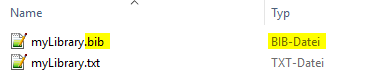
\includegraphics[width=.75\textwidth]{../../texfiles-beamer/tex-material/WissArb-latex/bib_txtDateien}
\end{figure}

\end{frame}

%%%%%%%%%%%%%%%%%%%%%%%%%%%%%%%%%%
\begin{frame}[fragile]
%\frametitle{Bibliographiedatenbank}

\begin{itemize}
	\item In der Bibiographiedatenbank befindet sich die Information Ihrer Quellen. In dem folgenden Format: 
\end{itemize}

\begin{lstlisting}
@book{Knuth1986,
  address = {Boston, MA},
  publisher = {Addison-Wesley},
  author = {Knuth, Donald E.},
  title = {The TeXbook},
  year = {1986}
}
\end{lstlisting}

\pause

\begin{itemize}
	\item \lstinline|@book|: \textbf{Werktyp}
	\item \lstinline|{ }|: Die \textbf{Klammern} umgeben den gesamten Eintrag.
	\item \lstinline|Knuth1986|: \textbf{ID} für das Werk (\alert{einzigartig} in der Datenbank sein!)
	\item \lstinline|address|: Ort der Veröffentlichung
	\item Die einzelnen Informationspunkte haben immer die gleiche \textbf{Syntax}: \lstinline|Art der Information = {Information},|
\end{itemize}
\end{frame}


%%%%%%%%%%%%%%%%%%%%%%%%%%%%%%%%%%
\begin{frame}[fragile]
%\frametitle{Literaturangaben}

\begin{itemize}
	\item Die Datenbank können Sie \textbf{mit jedem beliebigen Texteditor} bearbeiten. 
	
	\item Verwenden Sie \ltxpack{TeXstudio} für die Bearbeitung Ihrer \ltxterm{.bib}-Datei, werden die verschiedenen Teile besonders \textbf{hervorgehoben}.
	

\end{itemize}

\begin{figure}
	\centering
	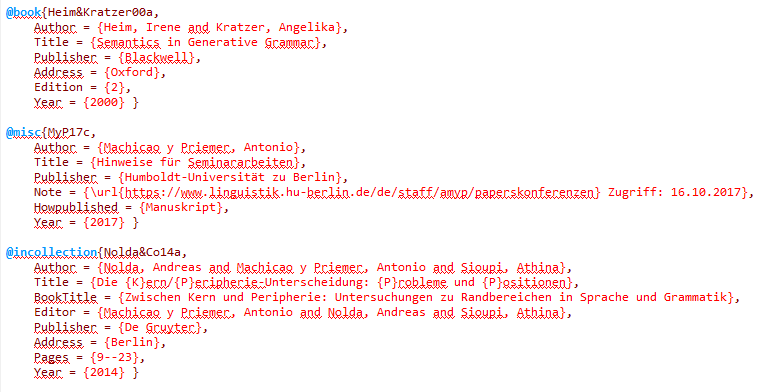
\includegraphics[width=.90\textwidth]{../../texfiles-beamer/tex-material/WissArb-latex/bibeintraege}
\end{figure}

\nocite{Heim&Kratzer00a}
\nocite{MyP17c}
\nocite{Nolda&Co14a}

\end{frame}


%%%%%%%%%%%%%%%%%%%%%%%%%%%%%%%%%%
\begin{frame}[fragile]
%\frametitle{Literaturangaben}

\begin{itemize}

	\item Ist die Datei in \ltxpack{TeXstudio} offen, werden die IDs bei der \textbf{Autovervollständigung} angezeigt.
\end{itemize}

\begin{figure}
	\centering
	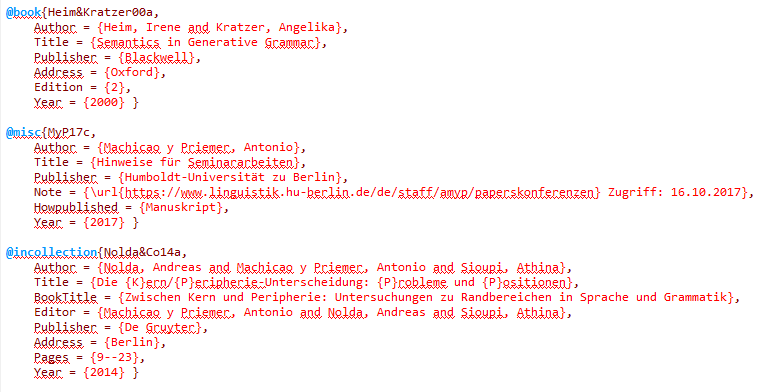
\includegraphics[width=.90\textwidth]{../../texfiles-beamer/tex-material/WissArb-latex/bibeintraege}
\end{figure}

\end{frame}


%%%%%%%%%%%%%%%%%%%%%%%%%%%%%%%%%%
\begin{frame}[fragile]
%\frametitle{Literaturangaben}


Die wichtigsten \textbf{Eintragstypen} sind:

\begin{enumerate}
	\item \textbf{\ltxterm{article}} für Zeitschriftenartikel
	\item \textbf{\ltxterm{book}} für veröffentlichte Bücher
	\item \textbf{\ltxterm{incollection}} für Artikel in Sammelbänden
	\item \textbf{\ltxterm{inproceedings}} für Artikel in Proceedings von Konferenzen
	\item \textbf{\ltxterm{phdthesis}} für Dissertationen
	\item \textbf{\ltxterm{unpublished}} für unveröffentlichte Manuskripte
	\item \textbf{\ltxterm{misc}} ein Joker, falls alles andere nicht passt
\end{enumerate}

\pause 

\begin{itemize}
	\item Eine Liste der \textbf{obligatorischen} und \textbf{optionalen Informationspunkte} je nach Eintrag finden Sie hier:
	
	\url{https://de.wikipedia.org/wiki/BibTeX}
	
	\item Weitere Informationen zu Bib\TeX\ finden Sie hier:
	
	\url{www.bibtex.org}
\end{itemize}

\end{frame}


%%%%%%%%%%%%%%%%%%%%%%%%%%%%%%%%%%
%%%%%%%%%%%%%%%%%%%%%%%%%%%%%%%%%%
\section{Angeben der Quellen}
\frame{
	\frametitle{~}
	\begin{multicols}{2}
		\tableofcontents[currentsection,hideallsubsections]
	\end{multicols}
}
%%%%%%%%%%%%%%%%%%%%%%%%%%%%%%%%%%

\begin{frame}[fragile]
\frametitle{Angeben der Quellen}

Eine Literaturangabe funktioniert im Prinzip genau so wie der Befehl \ltxterm{ref} bei Querverweisen, nur \textbf{mit dem Befehl \ltxterm{cite}} und mit der vergebenen \textbf{ID des Werks}:

\begin{lstlisting}
\cite{ID}
\end{lstlisting}

\pause

\vspace{.3cm}

Wenn eine Quelle \textbf{im Literaturverzeichnis erscheinen} soll, aber Sie die \textbf{Quelle nicht im Fließtext} angeben wollen, dann verwenden Sie den Befehl \textbf{\ltxterm{nocite}} mit der ID des Werks:

\begin{lstlisting}
\nocite{ID}
\end{lstlisting}

\end{frame}


%%%%%%%%%%%%%%%%%%%%%%%%%%%%%%%%%%
\begin{frame}[fragile]
%\frametitle{Literaturangaben}

Hier ein Beispiel wie Bib\TeX\ im Fließtext verwendet wird:

\begin{lstlisting}
Die folgende Angabe erscheint im Fließtext und in der 
Literaturliste (s.~Ende dieses Dokuments): \cite{Loebner15a}.
Diese Angabe erscheint dagegen nicht im Fließtext, aber in der 
Literaturliste (s.~Ende dieses Dokuments): 
\nocite{ZimmermannT&Sternefeld13a}
\end{lstlisting}

\outputbox{
Die folgende Angabe erscheint im Fließtext und in der 
Literaturliste (s.~Ende dieses Dokuments): \cite{Loebner15a}.
Diese Angabe erscheint dagegen nicht im Fließtext, aber in der 
Literaturliste (s.~Ende dieses Dokuments): 
\nocite{ZimmermannT&Sternefeld13a}
}


\end{frame}


%%%%%%%%%%%%%%%%%%%%%%%%%%%%%%%%%%
%%%%%%%%%%%%%%%%%%%%%%%%%%%%%%%%%%
\section{Bibliographiestil und Print-Befehl}
\frame{
	\frametitle{~}
	\begin{multicols}{2}
		\tableofcontents[currentsection,hideallsubsections]
	\end{multicols}
}
%%%%%%%%%%%%%%%%%%%%%%%%%%%%%%%%%%

\begin{frame}[fragile]
\frametitle{Bibliographiestil und Print-Befehl}

\begin{itemize}
	\item Das Aussehen des \textbf{Literaturverzeichnisses} und der im Fließtext angegebenen \textbf{Quellen} hängt vom \textbf{Bibliographiestil} ab.
	
	\item[]
	
	\item Die folgenden Stile sind immer vorhanden:
	
	\begin{itemize}
		\item \ltxterm{alpha}
		\item \ltxterm{abbrv}
		\item \ltxterm{plain}
		\item \ltxterm{unsrt}
	\end{itemize}

	\item[]
	
	\item Die Stile sind \idR für das Englische geschrieben. Im Netz finden Sie andere Stile für das Deutsche.
\end{itemize}

\end{frame}


%%%%%%%%%%%%%%%%%%%%%%%%%%%%%%%%%%
\begin{frame}[fragile]
%\frametitle{Bibliographiestil und Print-Befehl}

\begin{itemize}	
	\item Am \textbf{Ende des Dokuments} (oder an der \textbf{Position, an der die Literaturliste erscheinen soll}) wird die \textbf{Verlinkung zur eigenen Bibliographiedatenbank} erstellt. Das Literaturverzeichnis wird an dieser Stelle gedruckt.
		
	\item Es ist empfehlenswert den \textbf{Bibliographiestil} an der gleichen Stelle \textbf{festzulegen}.

\end{itemize}

\begin{lstlisting}
\bibliographystyle{Stilname}                % Bibliographiestil
\bibliography{.bib-Datei-Name} % Verlinkung zur Datenbank
                                            % (Druckbefehl)
\end{lstlisting}
\end{frame}


%%%%%%%%%%%%%%%%%%%%%%%%%%%%%%%%%%
\begin{frame}[fragile]
\frametitle{Stil: alpha}

\begin{figure}
	\centering
	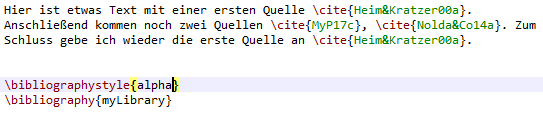
\includegraphics[width=.70\textwidth]{../../texfiles-beamer/tex-material/WissArb-latex/bib_alpha_tex}
\end{figure}

\begin{figure}
	\centering
	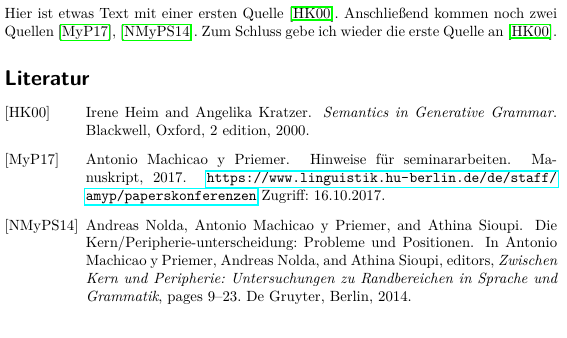
\includegraphics[width=.70\textwidth]{../../texfiles-beamer/tex-material/WissArb-latex/bib_alpha_pdf}
\end{figure}

\end{frame}


%%%%%%%%%%%%%%%%%%%%%%%%%%%%%%%%%%
\begin{frame}[fragile]
\frametitle{Stil: abbrv}

\begin{figure}
	\centering
	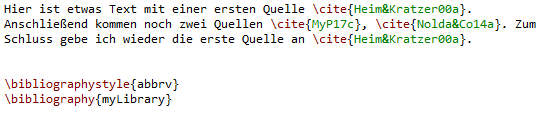
\includegraphics[width=.70\textwidth]{../../texfiles-beamer/tex-material/WissArb-latex/bib_abbrv_tex}
\end{figure}

\begin{figure}
	\centering
	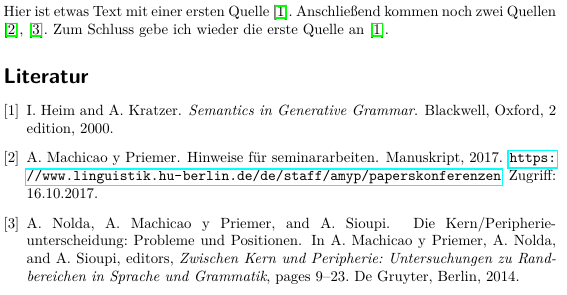
\includegraphics[width=.70\textwidth]{../../texfiles-beamer/tex-material/WissArb-latex/bib_abbrv_pdf}
\end{figure}

\end{frame}


%%%%%%%%%%%%%%%%%%%%%%%%%%%%%%%%%%
\begin{frame}[fragile]
\frametitle{Stil: plain}

\begin{figure}
	\centering
	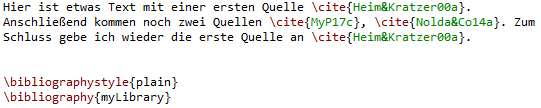
\includegraphics[width=.70\textwidth]{../../texfiles-beamer/tex-material/WissArb-latex/bib_plain_tex}
\end{figure}

\begin{figure}
	\centering
	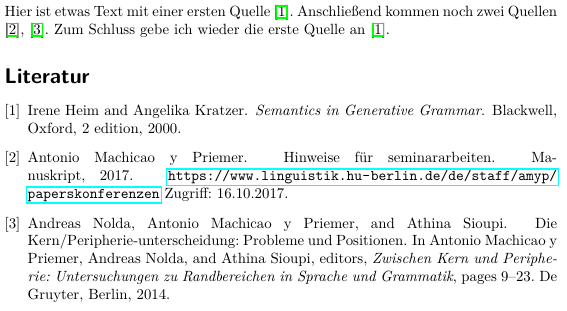
\includegraphics[width=.70\textwidth]{../../texfiles-beamer/tex-material/WissArb-latex/bib_plain_pdf}
\end{figure}

\end{frame}


%%%%%%%%%%%%%%%%%%%%%%%%%%%%%%%%%
%%%%%%%%%%%%%%%%%%%%%%%%%%%%%%%%%
\section{Das natbib-Paket}
\frame{
	\frametitle{~}
	\begin{multicols}{2}
		\tableofcontents[currentsection,hideallsubsections]
	\end{multicols}
}
%%%%%%%%%%%%%%%%%%%%%%%%%%%%%%%%%%

\begin{frame}[fragile]
\frametitle{Das natbib-Paket}

\begin{itemize}
	\item Das \ltxterm{natbib}-Paket bietet eine große Breite an Funktionen \citep[vgl.][]{Daly10a}. 
	
	\item[]
	
	\item Um den in der Linguistik häufig benutzten \textbf{\ltxterm{author(year)}-Stil} zu verwenden, sollte das Paket mit dieser \textbf{Option} geladen werden:

\begin{lstlisting}
\usepackage[authoryear]{natbib}
\end{lstlisting}
	
	\item[]
	
	\item Dafür sollte dementsprechend ein \textbf{\ltxterm{bibliographystyle}} ausgewählt werden, welcher mit der \ltxterm{author(year)}-Notation arbeitet, \zB \ltxterm{chicago} oder \ltxterm{apalike}.

\end{itemize}
\end{frame}


%%%%%%%%%%%%%%%%%%%%%%%%%%%%%%%%%%%
\begin{frame}[fragile]

\begin{itemize}
	\item Hier die in unserer Präambel geladenen Pakete bisher:
\end{itemize}

\begin{figure}
	\centering
	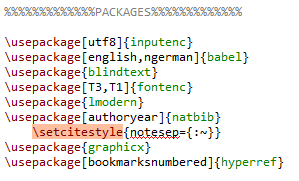
\includegraphics[width=.70\textwidth]{../../texfiles-beamer/tex-material/WissArb-latex/preamble3}
\end{figure}


\end{frame}

%%%%%%%%%%%%%%%%%%%%%%%%%%%%%%%%%%%
\begin{frame}[fragile]
\begin{itemize}
	\item Das \ltxterm{natbib}-Paket bietet \textbf{weitere Befehle} für Literaturverweise mit Klammern:


\begin{multicols}{2}
%\small	
	
\begin{lstlisting}
\citet{Knuth1986}
\citet[36]{Knuth1986}
\citet[vgl.][36]{Knuth1986}% ?
\citep{Knuth1986}
\citep[36]{Knuth1986}
\citep[vgl.][36]{Knuth1986}
\citep[vgl.][]{Knuth1986}
\end{lstlisting}

Knuth (1986)\\
Knuth (1986, 36)\\
Knuth (vgl.\ 1986, 36)\\
(Knuth, 1986)\\
(Knuth, 1986, 36)\\
(vgl.\ Knuth, 1986, 36)\\
(vgl.\ Knuth, 1986)\\
%\citet{Knuth1986}\newline 
%\citet[36]{Knuth1986}\newline
%\citet[vgl.][36]{Knuth1986}\newline  % ?
%\citep{Knuth1986}\newline 
%\citep[36]{Knuth1986}\newline
%\citep[vgl.][36]{Knuth1986}\newline 
%\citep[vgl.][]{Knuth1986}\newline
\end{multicols}

\end{itemize}

\pause

\begin{itemize}
	\item Um zwischen Jahres- und Seitenzahl einen \textbf{Doppelpunkt statt eines Kommas} zu verwenden, können \textbf{Spezifikationen zum Stil} beim Laden des Pakets geladen werden: 
\begin{lstlisting}
\usepackage[authoryear]{natbib}
	\setcitestyle{notesep={:~}}
\end{lstlisting}

\end{itemize}

\end{frame}


%%%%%%%%%%%%%%%%%%%%%%%%%%%%%%%%%%%
\begin{frame}[fragile]
%\frametitle{Literaturangaben}


\begin{lstlisting}
\usepackage[authoryear]{natbib}
\setcitestyle{notesep={:~}}
\end{lstlisting}

\footnotesize

\begin{tabular}{lll}
	\textbf{Code}                               & \textbf{Doppelpunkt}            & \textbf{Komma} \\
	
	\lstinline|\citet{Knuth1986}|               & \citet{Knuth1986}               & Knuth (1986)   \\
	
	\lstinline|\citet[36]{Knuth1986}|           & \citet[36]{Knuth1986}           & Knuth (1986, 36)   \\
	
	\lstinline|\citet[vgl.][36]{Knuth1986}| & \citet[vgl.][36]{Knuth1986} & Knuth (vgl.\ 1986, 36)  \\
	
	\lstinline|\citep{Knuth1986}|               & \citep{Knuth1986}               & (Knuth, 1986)   \\
	
	\lstinline|\citep[36]{Knuth1986}|     & \citep[36]{Knuth1986}           & (Knuth, 1986, 36) \\
	
	\lstinline|\citep[vgl.][36]{Knuth1986}|       & \citep[vgl.][36]{Knuth1986}     & (vgl.\ Knuth, 1986, 36)   \\
	
	\lstinline|\citep[vgl.][]{Knuth1986}|           & \citep[vgl.][]{Knuth1986}       & (vgl.\ Knuth, 1986)
\end{tabular}

\end{frame}


%%%%%%%%%%%%%%%%%%%%%%%%%%%%%%%%%%
\begin{frame}[fragile]
%\frametitle{Literaturangaben}

\noindent Hier einige Beispiele für \textbf{Literaturverweise ohne Klammern}:

\begin{multicols}{2}
\begin{lstlisting}
\citealt{Knuth1986}
\citealp{Knuth1986}
\end{lstlisting}
\citealt{Knuth1986}\newline
\citealp{Knuth1986}
\end{multicols}


\pause 


\noindent Hier einige Beispiele um nur \textbf{Teile der Information} zu erhalten:

\begin{multicols}{2}
\begin{lstlisting}
\citeauthor{Knuth1986}
\citeyear{Knuth1986}
\citeyearpar{Knuth1986}
\end{lstlisting}
\citeauthor{Knuth1986}\newline
\citeyear{Knuth1986}\newline
\citeyearpar{Knuth1986}
\end{multicols}

\end{frame}


%%%%%%%%%%%%%%%%%%%%%%%%%%%%%%%%%%
\begin{frame}[fragile]
%\frametitle{Literaturangaben}

\noindent Diese Befehle können bspw.\ verwendet werden, um Verweise in Genitiv zu setzen:

\begin{lstlisting}
\dots\ wie in 
\citeauthor{Knuth1986}s \citeyearpar{Knuth1986}
Buch bereits gesehen \dots\
\end{lstlisting}
\outputbox{
\dots\ wie in 
\citeauthor{Knuth1986}s \citeyearpar{Knuth1986}
Buch bereits gesehen \dots\ 
}

\end{frame}


%%%%%%%%%%%%%%%%%%%%%%%%%%%%%%%%%%
\begin{frame}[fragile]
%\frametitle{Literaturangaben}

Um \textbf{mehr als eine Quelle} zu zitieren, gibt man sie einfach getrennt durch Kommata an:

\begin{lstlisting}
Hier ist ein Verweis mit drei Namen
\citep[vgl.][]{Knuth1986,Rothstein11a,Meindl11a}.
\end{lstlisting}

\outputbox{
Hier ist ein Verweis mit drei Namen
\citep[vgl.][]{Knuth1986,Rothstein11a,Meindl11a}.
}
\vspace{1em}


\pause 


Bib\TeX\ \textbf{kürzt} automatisch die Literaturverweise mit \gqq{\textbf{et al.}}, wenn dort \textbf{mehr als zwei Namen} vorhanden sind.

\begin{lstlisting}
Hier ist eine Quelle, die drei Namen enthält
\citep[vgl.][]{Nolda&Co14a}.
\end{lstlisting}

\outputbox{
Hier ist eine Quelle, die drei Namen enthält
\citep[vgl.][]{Nolda&Co14a}.
}

\end{frame}



%%%%%%%%%%%%%%%%%%%%%%%%%%%%%%%%%%
\begin{frame}[fragile]
\frametitle{Stil: apalike}


\begin{figure}
	\centering
	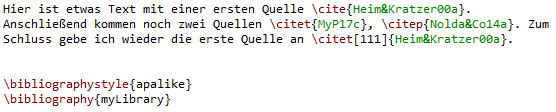
\includegraphics[width=.70\textwidth]{../../texfiles-beamer/tex-material/WissArb-latex/bib_apalike_tex}
\end{figure}

\begin{figure}
	\centering
	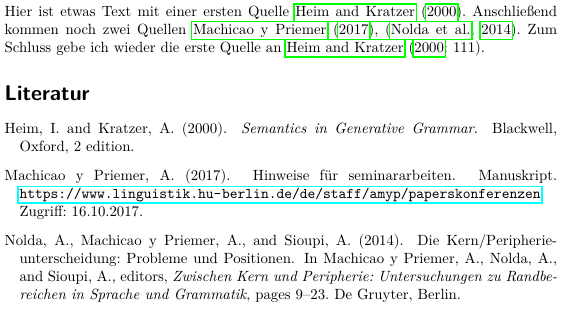
\includegraphics[width=.70\textwidth]{../../texfiles-beamer/tex-material/WissArb-latex/bib_apalike_pdf}
\end{figure}

\end{frame}


%%%%%%%%%%%%%%%%%%%%%%%%%%%%%%%%%%
\begin{frame}[fragile]
\frametitle{Stil: chicago}


\begin{figure}
	\centering
	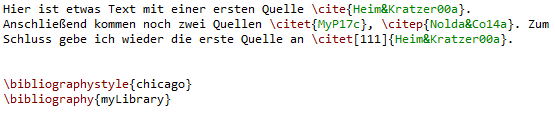
\includegraphics[width=.70\textwidth]{../../texfiles-beamer/tex-material/WissArb-latex/bib_chicago_tex}
\end{figure}

\begin{figure}
	\centering
	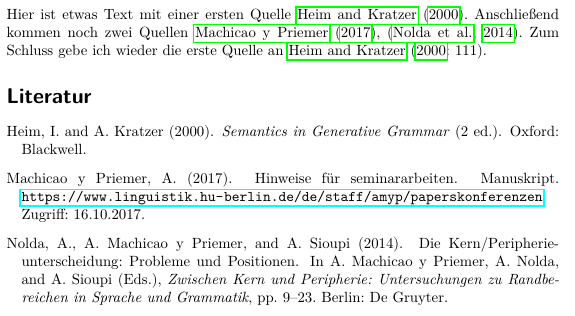
\includegraphics[width=.70\textwidth]{../../texfiles-beamer/tex-material/WissArb-latex/bib_chicago_pdf}
\end{figure}

\end{frame}


%%%%%%%%%%%%%%%%%%%%%%%%%%%%%%%%%%
\begin{frame}[fragile]
\frametitle{Stil: chicago auf Deutsch}

\begin{itemize}	
	\item Eine Version des \ltxterm{chicago}-Stils für das Deutsche angepasst (\ltxterm{deChicagoMyP}) finden Sie im Moodlekurs. Speichern Sie die Datei \ltxterm{deChicagoMyP.bst} \textbf{in dem gleichen Ordner} wie Ihre \ltxterm{.tex}-Datei und verwenden Sie den Stil wie immer:
\end{itemize}

\begin{figure}
	\centering
	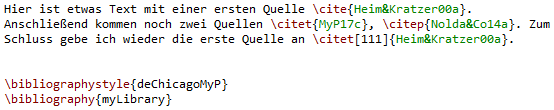
\includegraphics[width=.70\textwidth]{../../texfiles-beamer/tex-material/WissArb-latex/bib_deChicago_tex}
\end{figure}

%\begin{figure}
%	\centering
%	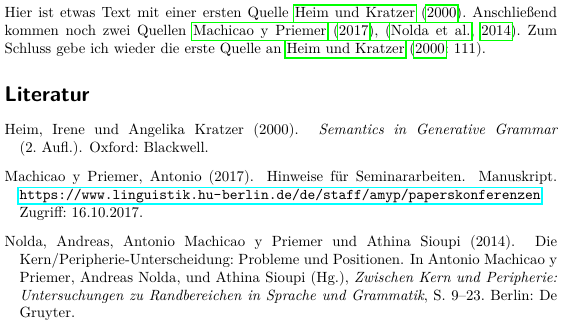
\includegraphics[width=.70\textwidth]{../../texfiles-beamer/tex-material/WissArb-latex/bib_deChicago_pdf}
%\end{figure}

\end{frame}


%%%%%%%%%%%%%%%%%%%%%%%%%%%%%%%%%%
\begin{frame}[fragile]
\frametitle{Stil: deChicagoMyP}

\begin{figure}
	\centering
	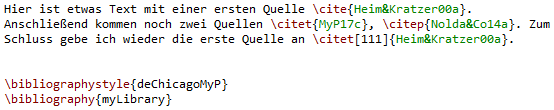
\includegraphics[width=.70\textwidth]{../../texfiles-beamer/tex-material/WissArb-latex/bib_deChicago_tex}
\end{figure}

\begin{figure}
	\centering
	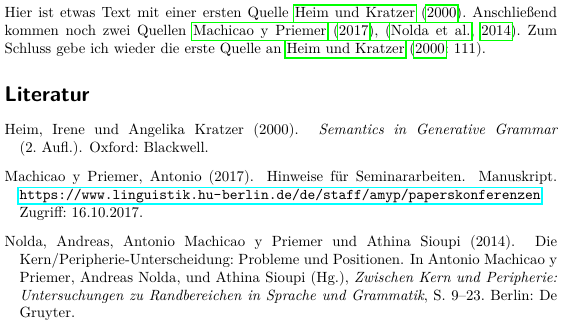
\includegraphics[width=.70\textwidth]{../../texfiles-beamer/tex-material/WissArb-latex/bib_deChicago_pdf}
\end{figure}

\end{frame}


%%%%%%%%%%%%%%%%%%%%%%%%%%%%%%%%%%
%%%%%%%%%%%%%%%%%%%%%%%%%%%%%%%%%%
\section{Quellenangaben als Links}
\frame{
	\frametitle{~}
	\begin{multicols}{2}
		\tableofcontents[currentsection,hideallsubsections]
	\end{multicols}
}
%%%%%%%%%%%%%%%%%%%%%%%%%%%%%%%%%%

\begin{frame}[fragile]
\frametitle{Quellenangaben als Links}

\begin{itemize}
	\item Quellenangaben können in Dokumenten als \textbf{aktive Links} verwendet werden. Dafür wird das \textbf{Paket \ltxterm{hyperref}} verwendet.
	
	\item[]
	
	\item Wenn man auf die Quelle in der PDF-Datei klickt, kommt man zu dem Eintrag im Literaturverzeichnis.
	
	\item[]	
	\item Mit der \textbf{Option \ltxterm{hidelinks}} wird bei der PDF die \textbf{Umrandung} der Links unterbunden (Die Links bleiben aktiv!). Die farbige Umrandung der Links erscheint nur auf der PDF, nicht beim Druck! 
	
	\lstinline|\usepackage[bookmarksnumbered, hidelinks]{hyperref}|
\end{itemize}

\end{frame}


%%%%%%%%%%%%%%%%%%%%%%%%%%%%%%%%%%
%%%%%%%%%%%%%%%%%%%%%%%%%%%%%%%%%%
\section{Kompilierungsprozess \& Fehler}
\frame{
	\frametitle{~}
	\begin{multicols}{2}
		\tableofcontents[currentsection,hideallsubsections]
	\end{multicols}
}
%%%%%%%%%%%%%%%%%%%%%%%%%%%%%%%%%%

\begin{frame}[fragile]
\frametitle{Kompilierungsprozess \& Fehler}

Damit ein Literaturverzeichnis erstellt wird, ist es notwendig das Dokument \textbf{mehrmals zu kompilieren}:

\begin{enumerate}
	\item kompilieren mit \textbf{\ltxterm{PDFLaTeX}}, um die Literaturangaben zu finden (und in die \ltxterm{.aux}-Datei zu speichern),

\pause
	
	\item kompilieren mit \textbf{\ltxterm{BibTeX}}, um die Literaturangaben aus der \ltxterm{.aux}-Datei mit denen aus der \ltxterm{.bib}-Datei zu vergleichen (es wird eine \ltxterm{.bbl}-Datei generiert),

\pause
	
	\item kompilieren mit \textbf{\ltxterm{PDFLaTeX}}, um Literaturangaben einzusetzen und die Bibliographie (aus der \ltxterm{.bbl}-Datei) zu erstellen,

\pause
	
	\item kompilieren mit \textbf{\ltxterm{PDFLaTeX}}, falls die Literaturangaben oder die Bibliographie die Seitenzahlen des Dokuments geändert haben.

\pause
	
	\item[=] \ltxterm{PDFLaTeX} $+$ \ltxterm{BibTeX} $+$ \ltxterm{PDFLaTeX} $+$ \ltxterm{PDFLaTeX}
\end{enumerate}

\end{frame}


%%%%%%%%%%%%%%%%%%%%%%%%%%%%%%%%%%
\begin{frame}[fragile]
%\frametitle{Kompilierungsprozess}

\begin{itemize}
	\item Manchmal sind Bib\TeX -Fehler so schwerwiegend, dass Sie Ihre \textbf{Hilfsdateien löschen} müssen, damit das Dokument wieder kompiliert.
	
	(Löschen Sie \textbf{nicht} die \ltxterm{mydocument.tex}- und die   \ltxterm{mylibrary.bib}-Datei. Das sind keine Hilfsdateien.)
\end{itemize}
	

\begin{block}{Hilfsdateien}
	Hilfsdateien sind die Dateien, die generiert werden, wenn Sie Ihre \ltxterm{.tex}-Datei kompilieren: \ltxterm{mydocument.aux}, \ltxterm{mydocument.bbl}, \ltxterm{mydocument.log}, usw.
\end{block}

\end{frame}


%%%%%%%%%%%%%%%%%%%%%%%%%%%%%%%%%%
\begin{frame}
%\frametitle{Kompilierungsprozess}

\begin{itemize}	
	\item \textbf{Typische Fehler} bei Bib\TeX :
	
	\begin{itemize}
		\item In der \ltxterm{.bib}-Datei wurde ein \textbf{Komma} oder eine \textbf{Klammer} vergessen.
		
		\item[]
		
		\item In Ihrer \ltxterm{.bib}-Datei wurde ein \textbf{Sonderzeichen}, \zB \& benutzt, ohne \textbackslash  zu schreiben.
	\end{itemize} 

	\item[]
	
	\item TeXstudio hat eine Funktion um Hilfsdateien aufzuräumen:
	
	siehe: \texttt{Tools/Hilfsdateien aufräumen}
\end{itemize}

\end{frame}


%%%%%%%%%%%%%%%%%%%%%%%%%%%%%%%%%%
\begin{frame}[fragile]
%\frametitle{Kompilierungsprozess}

\begin{itemize}
	\item Namen, die mit \textbf{Sonderzeichen} (oder Akzente) beginnen (\zB \v{Z}ivanović mit Hatschek \v{} auf dem \emph{Z}) werden in der Literaturliste manchmal \textbf{nicht korrekt eingeordnet}.
\end{itemize}

\begin{figure}
	\centering
	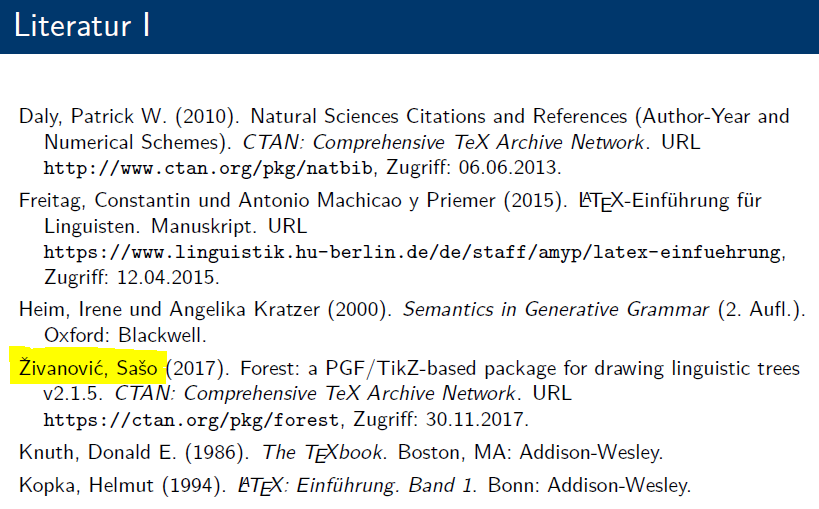
\includegraphics[scale=.4]{../../texfiles-beamer/tex-material/WissArb-latex/bib-Liste-false1}
\end{figure}

\nocite{WieseB11a}
\nocite{Zivanovic17a}

\end{frame}


%%%%%%%%%%%%%%%%%%%%%%%%%%%%%%%%%%
\begin{frame}[fragile]
%\frametitle{Kompilierungsprozess}

\begin{itemize}
	\item Für eine korrekte Einordnung muss der Code für solche Sonderzeichen angegeben werden, d.\,h. \lstinline|\v{Z}| für \v{Z}.
\end{itemize}

\begin{figure}
	\centering
	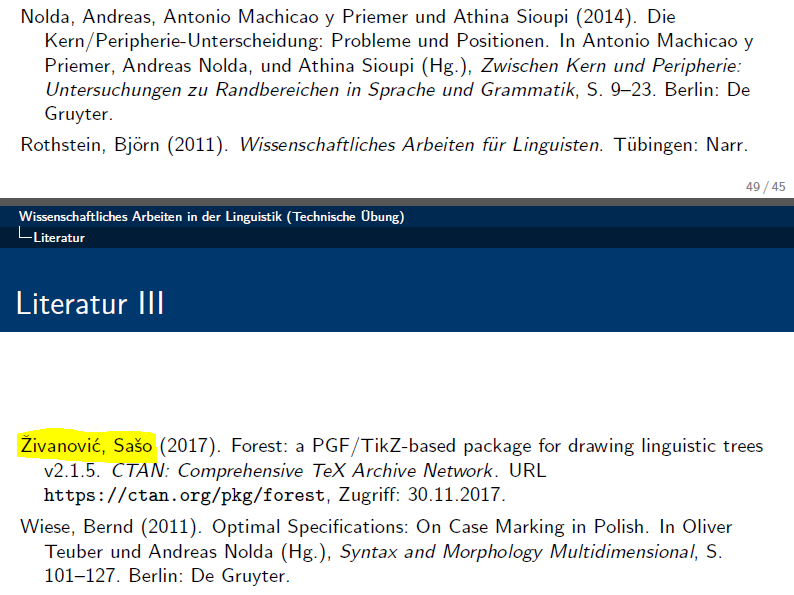
\includegraphics[scale=.4]{../../texfiles-beamer/tex-material/WissArb-latex/bib-Liste-false2}
\end{figure}


\end{frame}


%%%%%%%%%%%%%%%%%%%%%%%%%%%%%%%%%%
\begin{frame}[fragile]
%\frametitle{Kompilierungsprozess}

\begin{itemize}
	\item Nun wird aber \v{Z}ivanovi{\'c} unter \textbf{v} eingeordnet. Die korrekte Einordnung erfolgt dadurch, dass \lstinline|\v{Z}| in geschweiften Klammern \textbf{geschützt} und damit als \textbf{ein} Buchstabe interpretiert wird \lstinline|{\v{Z}}|. 
\end{itemize}

\begin{figure}
	\centering
	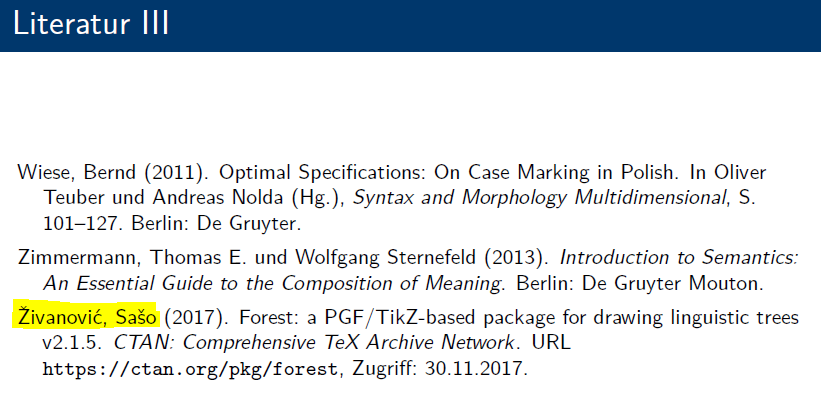
\includegraphics[scale=.4]{../../texfiles-beamer/tex-material/WissArb-latex/bib-Liste-right}
\end{figure}


\end{frame}	
	
%%%%%%%%%%%%%%%%%%%%%%%%%%%%%%%%%%%%%%%%%%%%%%%%%%%%%%%%%
%%%%%%%%%%%%%%%%%%%%%%%%%%%%%%%%%%%%%%%%%%%%%%%%%%%%%%%%

\section{Hausaufgabe}
\frame{
\begin{multicols}{2}
%\frametitle{~}
	\tableofcontents[currentsection,hideallsubsections]
\end{multicols}
}
%
%%%%%%%%%%%%%%%%%%%%%%%%%%%%%%%%%%%%%%%%%%%%%%%%%%%%%
\begin{frame}{Hausaufgabe 1}

\begin{itemize}
	
	\item Laden Sie folgende Dateien aus dem Moodlekurs herunter:
	
	\begin{enumerate}
		\item \ltxterm{myLibrary.txt}
		\item \ltxterm{test3PDF.pdf}
		\item \ltxterm{deChicagoMyP.bst}
	\end{enumerate}
	
	\item Ändern Sie die Endung von \ltxterm{myLibrary\alert{.txt}} in \ltxterm{myLibrary\alert{.bib}}
	
	\item Speichern Sie die heruntergeladenen Dateien \textbf{im gleichen Ordner} wie Ihre \ltxterm{.tex-Datei}

	
\end{itemize}

\end{frame}


%%%%%%%%%%%%%%%%%%%%%%%%%%%%%%%%%%%%%%%%%%%%%%%%%%%%
\begin{frame}[fragile]{Hausaufgabe 2}

\begin{itemize}
	
	\item Installieren Sie das folgende Paket in Ihrem \ltxterm{myName.tex}-Dokument (mit dem Befehl \ltxterm{usepackage}).
	
	\begin{itemize}
		\item \ltxterm{natbib}
	\end{itemize}
	
	\item[NB] Vergessen Sie nicht die \textbf{Option \ltxterm{authoryear}}, und ändern Sie die Spezifikation des Pakets von Kommatrennung auf \textbf{Doppelpunkttrennung}.

%	\item Ergänzen Sie die Option \ltxterm{hidelinks} für das Paket \ltxterm{hyperref}. Hier die Syntax dafür:
%		
%		\lstinline|\usepackage[bookmarksnumbered,hidelinks]{hyperref}|
%		
%	\item[NB] Bitte beachten Sie, dass \ltxterm{hyperref} als letztes Paket geladen werden sollte.
\end{itemize}

\end{frame}


%%%%%%%%%%%%%%%%%%%%%%%%%%%%%%%%%%%%%%%%%%%%%%%%%%%%%
\begin{frame}{Hausaufgabe 3}

\begin{itemize}
	
	\item Verwenden Sie Ihre \ltxterm{myName.tex}-Datei vom letzten Mal und geben Sie den benötigten Code ein, um das Ergebnis zu erhalten, das Sie in \ltxterm{test3PDF.pdf} sehen.
	
	\item[NB] Achten Sie darauf, dass es im ersten Absatz \textbf{drei verlinkte Quellenverweise} gibt!
	
	\item Dafür müssen Sie auch Information in Ihre \ltxterm{myLibrary.bib}-Datei eingeben!
	
	\item[NB] Achten Sie darauf, \textbf{wo} sich das Literaturverzeichnis befindet, und \textbf{welcher Stil} benutzt wird! 
\end{itemize}
\end{frame}


%%%%%%%%%%%%%%%%%%%%%%%%%%%%%%%%%%%%%%%%%%%%%%%%%%%%%
\begin{frame}{Hausaufgabe 4}

\begin{itemize}
		
	\item Laden Sie dann Ihre \texttt{myName.tex}-Datei, Ihre \ltxterm{myLibrary.bib}-Datei und Ihr PDF-Ergebnis bei Moodle hoch. 
	
	(Sie müssen nun 3 Dateien hochladen!)
	
	\item[NB:] Schauen Sie sich die Dokumentation des Pakets \ltxterm{natbib} an \citep{Daly10a}.
	
\end{itemize}

\end{frame}


%%%%%%%%%%%%%%%%%%%%%%%%%%%%%%%%%%%%%%%%%%%%%%%%%%%%%
\begin{frame}{Hausaufgabe -- Hinweise}

\begin{itemize}
	
	\item Es gibt einen YouTube-Channel mit \LaTeX -Tutorials:
	
	\url{https://www.youtube.com/channel/UCC-3dzj6dfbWwGzQzhkUS5A}
	
	\item Bei Twitter finden Sie tägliche \LaTeX -Tweets unter:
	
	\url{https://twitter.com/textip}
	
\end{itemize}

\end{frame}


%%%%%%%%%%%%%%%%%%%%%%%%%%%%%%%%%%%%%%%%%%%%%%%%%%%%%%%%%%
%%%%%%%%%%%%%%%%%%%%%%%%%%%%%%%%%%%%%%%%%%%%%%%%%%%%%%%%%

%\section{XY}
%%\frame{
%%\begin{multicols}{2}
%%\frametitle{~}
%%	\tableofcontents[currentsection]
%%\end{multicols}
%%}
%%
%%%%%%%%%%%%%%%%%%%%%%%%%%%%%%%%%%%%%%%%%%%%%%%%%%%%%
%
%\begin{frame}{XY}
%
%\begin{itemize}
%	\item XY
%\end{itemize}
%
%\end{frame}


%%%%%%%%%%%%%%%%%%%%%%%%%%%%%%%%%%%%%%%%%%%%%%%%%%%%%%%%%%
%%%%%%%%%%%%%%%%%%%%%%%%%%%%%%%%%%%%%%%%%%%%%%%%%%%%%%%%%

%\section{XY}
%%\frame{
%%\begin{multicols}{2}
%%\frametitle{~}
%%	\tableofcontents[currentsection]
%%\end{multicols}
%%}
%%
%%%%%%%%%%%%%%%%%%%%%%%%%%%%%%%%%%%%%%%%%%%%%%%%%%%%%
%
%\begin{frame}{XY}
%
%\begin{itemize}
%	\item XY
%\end{itemize}
%
%\end{frame}


%%%%%%%%%%%%%%%%%%%%%%%%%%%%%%%%%%%%%%%%%%%%%%%%%%%%%%%%%%
%%%%%%%%%%%%%%%%%%%%%%%%%%%%%%%%%%%%%%%%%%%%%%%%%%%%%%%%%

%\section{XY}
%%\frame{
%%\begin{multicols}{2}
%%\frametitle{~}
%%	\tableofcontents[currentsection]
%%\end{multicols}
%%}
%%
%%%%%%%%%%%%%%%%%%%%%%%%%%%%%%%%%%%%%%%%%%%%%%%%%%%%%
%
%\begin{frame}{XY}
%
%\begin{itemize}
%	\item XY
%\end{itemize}
%
%\end{frame}


%%%%%%%%%%%%%%%%%%%%%%%%%%%%%%%%%%%%%%%%%%%%%%%%%%%%%%%%%%
%%%%%%%%%%%%%%%%%%%%%%%%%%%%%%%%%%%%%%%%%%%%%%%%%%%%%%%%%

%\section{XY}
%%\frame{
%%\begin{multicols}{2}
%%\frametitle{~}
%%	\tableofcontents[currentsection]
%%\end{multicols}
%%}
%%
%%%%%%%%%%%%%%%%%%%%%%%%%%%%%%%%%%%%%%%%%%%%%%%%%%%%%
%
%\begin{frame}{XY}
%
%\begin{itemize}
%	\item XY
%\end{itemize}
%
%\end{frame}


%%%%%%%%%%%%%%%%%%%%%%%%%%%%%%%%%%%%%%%%%%%%%%%%%%%%%%%%%%
%%%%%%%%%%%%%%%%%%%%%%%%%%%%%%%%%%%%%%%%%%%%%%%%%%%%%%%%%

%\section{XY}
%%\frame{
%%\begin{multicols}{2}
%%\frametitle{~}
%%	\tableofcontents[currentsection]
%%\end{multicols}
%%}
%%
%%%%%%%%%%%%%%%%%%%%%%%%%%%%%%%%%%%%%%%%%%%%%%%%%%%%%
%
%\begin{frame}{XY}
%
%\begin{itemize}
%	\item XY
%\end{itemize}
%
%\end{frame}


%%%%%%%%%%%%%%%%%%%%%%%%%%%%%%%%%%%%%%%%%%%%%%%%%%%%
%%%                References                  
%%%%%%%%%%%%%%%%%%%%%%%%%%%%%%%%%%%%%%%%%%%%%%%%%%%% 

\appendix
\backupbegin


%%%%%%%%%%%%%%%%%%%%%%%%%%%%%%%%%%
%%%%%%%%%%%%%%%%%%%%%%%%%%%%%%%%%%
\section{Quellen}
%\frame{
%\begin{multicols}{2}
%\frametitle{~}
%	\tableofcontents[currentsection]
%\end{multicols}
%}
%%%%%%%%%%%%%%%%%%%%%%%%%%%%%%%%%%

\begin{frame}[allowframebreaks]
\frametitle{Quellen}

{\footnotesize
	
	\begin{itemize}
		%	\item \DWDS{1} \url{https://www.dwds.de/r?h=1&from=&corpus=kern&q=von+uns+gehen} \\
		%	{[}Zugriff: 10.04.2017]; Treffer aus: \citep[202]{Becker69a} 
		%	
		
%		\item Grafik: File Extensions -- xkcd, A webcomic of romance,
%		sarcasm, math, and language,
%		\url{https://xkcd.com/1301/} \\
%		{[}Zugriff: 10.04.2017]
%		

		\item Link: Bib\TeX\ -- Wikipedia\\
		\url{https://de.wikipedia.org/wiki/BibTeX}\\
		{[}Zugriff: 23.10.2017]
		
		\item Link: Bib\TeX .org\\
		\url{http://www.bibtex.org}\\
		{[}Zugriff: 23.10.2017]
		
		\item Link: Creating and Managing Bibliographies with Bib\TeX\ on Overleaf -- (Lian Tze Lim)\\
		\url{https://www.overleaf.com/blog/532-creating-and-managing-bibliographies-with-bibtex-on-overleaf}\\
		{[}Zugriff: 28.11.2017]
	
		\item Paket: \ltxpack{natbib} -- Flexible bibliography support.\\
		\url{https://ctan.org/pkg/natbib}\\
		{[}Zugriff: 23.10.2017]

		\item Twitter: \TeX\ tips\\
		\url{https://twitter.com/textip} \\
		{[}Zugriff: 10.04.2017]

		\item YouTube-Tutorial: \LaTeX\ Tutorial\\
		\url{https://www.youtube.com/channel/UCC-3dzj6dfbWwGzQzhkUS5A}\\
		{[}Zugriff: 23.10.2017]
		
%		\item Software: \ltxpack{TeXstudio}\\
%		\url{https://www.texstudio.org/} \\
%		{[}Zugriff: 10.04.2017]
		
%		\item Grafik: Kontextuelle Bedeutung: Wrong Hands -- John Atkinson, \url{http://wronghands1.tumblr.com/post/157354512780} \\
%		{[}Zugriff: 23.01.2017]
%		
%		\item Grafik: Ludwig Wittgenstein: von Moritz Nähr -- Austrian National Library, Gemeinfrei, \url{https://commons.wikimedia.org/w/index.php?curid=46116699} \\
%		{[}Zugriff: 11.04.2017]	
%		
%		\item Grafik: Semantics -- the dark side: mdhk, \url{http://mdhk.tumblr.com/post/78033341047/yes} \\
%		{[}Zugriff: 29.07.2016]
%		
%		\item Grafik: Semantische Restriktionen: Linguist Llama, \url{http://lingllama.tumblr.com/post/14266418758/picture-background-8-piece-pie-style-color} \\
%		{[}Zugriff: 07.04.2014]
%		
%		\item Video: Trump vs.\ Truth: Last Week Tonight with John Oliver (HBO) \url{https://www.youtube.com/watch?v=xecEV4dSAXE} \\
%		{[}Zugriff: 12.04.2017]
		
	\end{itemize}
}

\end{frame}
%%%%%%%%%%%%%%%%%%%%%%%%%%%%%%%%%%


%%%%%%%%%%%%%%%%%%%%%%%%%%%%%%%%%%
%%%%%%%%%%%%%%%%%%%%%%%%%%%%%%%%%%
\section{Literatur}
%\frame{
%\begin{multicols}{2}
%\frametitle{~}
%	\tableofcontents[currentsection]
%\end{multicols}
%}
%%%%%%%%%%%%%%%%%%%%%%%%%%%%%%%%%%

\begin{frame}[allowframebreaks]
\frametitle{Literatur}

%German
\bibliographystyle{../../texfiles-beamer/deChicagoMyP}

%	%English
%	\bibliographystyle{../../texfiles-beamer/enChicagoMyP} 


{\footnotesize
	\bibliography{../../texfiles-beamer/tex-literature}
}	
\end{frame}
%%%%%%%%%%%%%%%%%%%%%%%%%%%%%%%%%%

\backupend

\end{document}
